%!TEX root = ../thesis.tex
%*******************************************************************************
%*********************************** First Chapter *****************************
%*******************************************************************************

\chapter{Design - COVID Moonshot}
As COVID-19 infections swept through the globe in March 2020, the COVID Moonshot program was established by an international group of scientists to search for potent drugs against COVID-19. The initiative was precipitated by the release of data from a large XChem crystallographic fragment screen conducted at Diamond, which yielded over 60 fragment hits against the SARS-CoV-2 main protease (MPro) complete with detailed structures of fragment-protein complexes. As SARS-CoV-2 Mpro is vital for the replication of the virus, it is one of the most promising protein targets for anti-viral therapeutics. 

COVID Moonshot was then set up as a fully-open crowdsourcing and crowdfunding endeavor, inviting new inhibitors designs based on these initial fragment hits from the scientific community. Submitted inhibitor designs are triaged based on diversity and synthesizability, with synthesis routes generated by an ML workflow based on the Molecular Transformer (as discussed in Chapter 2). Compounds are then ordered and synthesized commercially before being assayed for activity by research groups around the world. At the time of writing this open-source design-make-test cycle is ongoing, with over 900 compounds have been made and tested.

This chapter details my contribution to the project at two different stages: (i) attempting to generate fragment merges using a genetic algorithm based on SOAP descriptors, and (ii) optimising a chemical series by learning the ranking of activity from assay data using a siamese graph network and screening a constructed library. From (ii) I have generated and submitted 6 candidate designs which are currently being synthesized.

\section{Fragment merging}
Having found multiple fragment hits, the immediate next step was to propose additions to the small molecular fragments in order to increase potency. This is the standard methodology in fragment-based drug design (Fig \ref{fig:frag}), where fragments are often merged/linked together usually by inspecting the geometrical complementarity between the crystal structures of the bound fragment-protein complexes. Common proposals attempt to identify overlapping aromatic ring structures between two fragments which can therefore be straightforwardly merged.

\begin{figure}[!h] % !h ~ force here, t ~ top, b ~ bottom, p ~ separate page
\centering
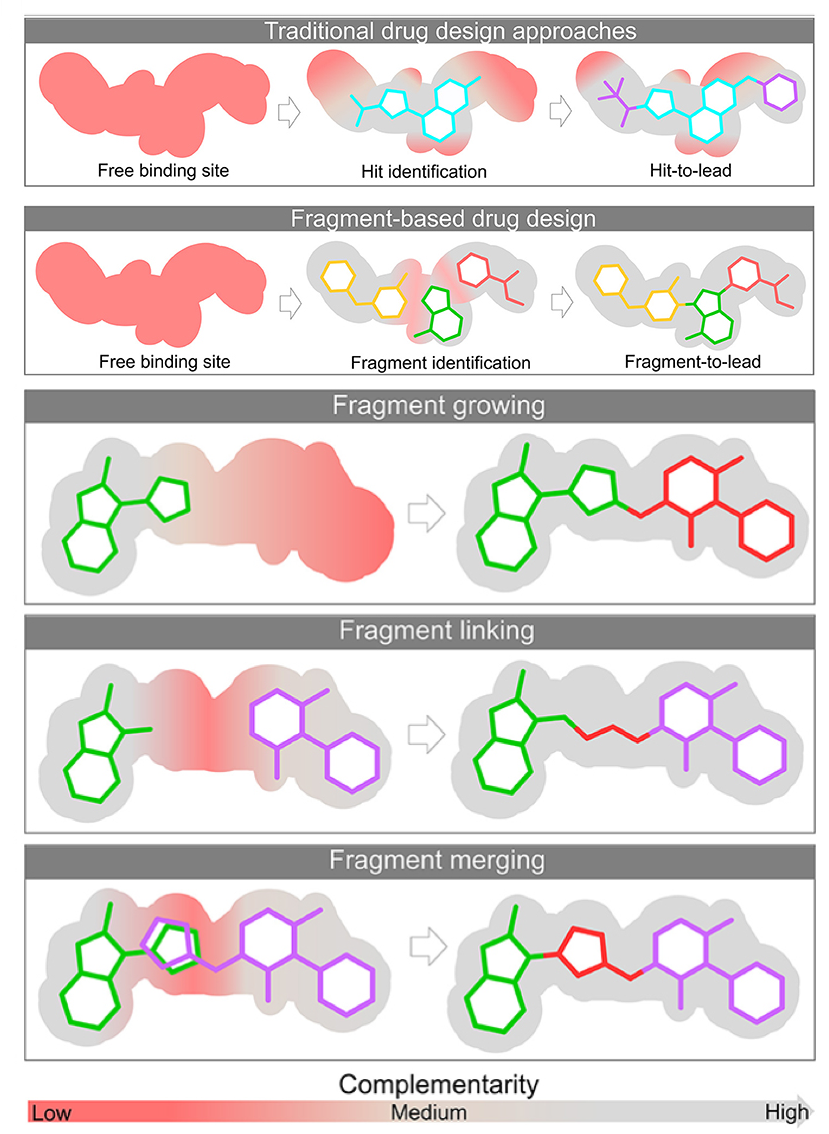
\includegraphics[width=0.7\textwidth]{Chapter3/Figs/frag_design.png}
\caption{\label{fig:frag} An illustration of fragment-based drug design. Diagram adapted from \cite{fragpic}.}
\end{figure}

Given the rich crystallographic spatial data available, as well as the inherently geometrical nature of the problem, it seemed natural to approach this task using a precise feature of molecular shape - SOAP. Instead of property prediction, the objective was to identify molecular candidates with shapes that are the most complementary to the atomic arrangement of the fragments in the binding site. With this in mind, a genetic algorithm (GA) approach was chosen.

GAs are particularly useful for situation where no efficient deterministic algorithms are available, which was the case for this problem. GAs are inspired by natural selection, involving the generational evolution and mutation of a population towards increasing fitness. Defining mutations and evolutionary mating in chemical space can be done by representing molecules as graphs \cite{Jensen19}: possible mutations involve the modification of atoms and bonds, such as the insertion/deletion of atoms, changes in bond order, and closing/opening of rings, while mating of candidates are done via the cutting and subsequent joining of chemical bonds (Fig.\ref{fig:GBGA}).

\begin{figure}[!h] % !h ~ force here, t ~ top, b ~ bottom, p ~ separate page
\centering
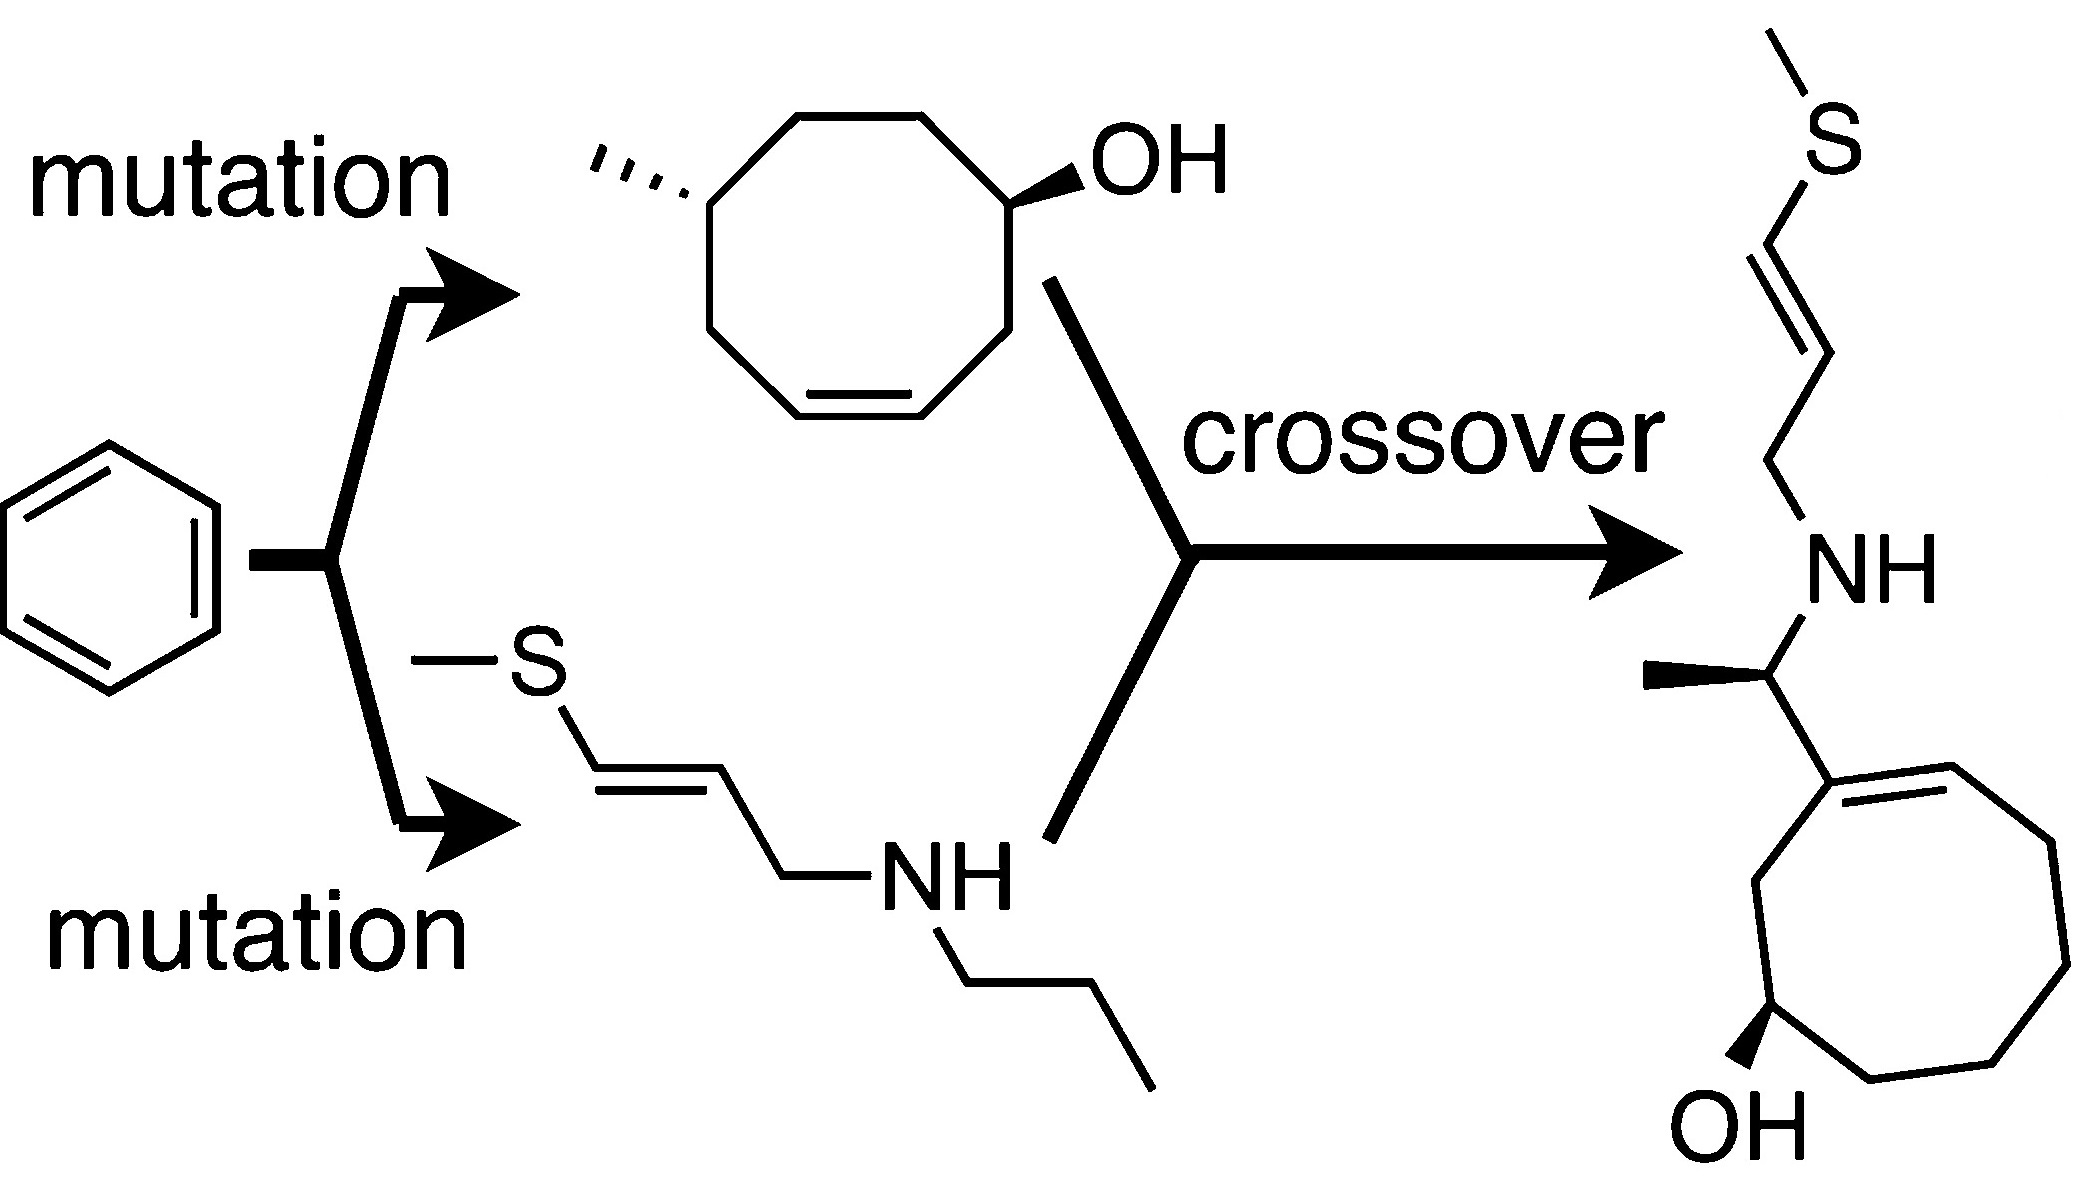
\includegraphics[width=0.45\textwidth]{Chapter3/Figs/GBGA.jpeg}
\caption{\label{fig:GBGA} A graphical illustration of a molecule mutating and mating through a genetic algorithm. Figure reproduced from \cite{Virshup13}.}
\end{figure}

The SOAP descriptor for a molecular graph can be calculated as before by generating a conformer for the molecule represented by the graph. The fitness function for evolving the GA must measure the shape complementarity of a molecule with the fragment coordinates - an obvious choice would be the SOAP similarity kernel between the molecule and the SOAP vector that is generated by considering the atomic coordinates of all of the fragments in the binding site. Conceptually, one could visualise this as attempting to find the SOAP vector that best aligns with the SOAP `field' constructed from the orientations of the bound fragments. The 66 discovered fragment hits are divided between two different binding sites of the MPro protein, so two separate GAs are implemented, with the 66 fragment hits serving as the initial population for the algorithm.

$\sim$200 runs of each of the two GAs were executed, and the resultant top-scoring candidates underwent rudimentary filtering for chemical reasonableness by eye. 37 molecular candidates (Fig. \ref{fig:GA_subs}) were eventually submitted to the COVID Moonshot team. 

\begin{figure}[!h] % !h ~ force here, t ~ top, b ~ bottom, p ~ separate page
\centering
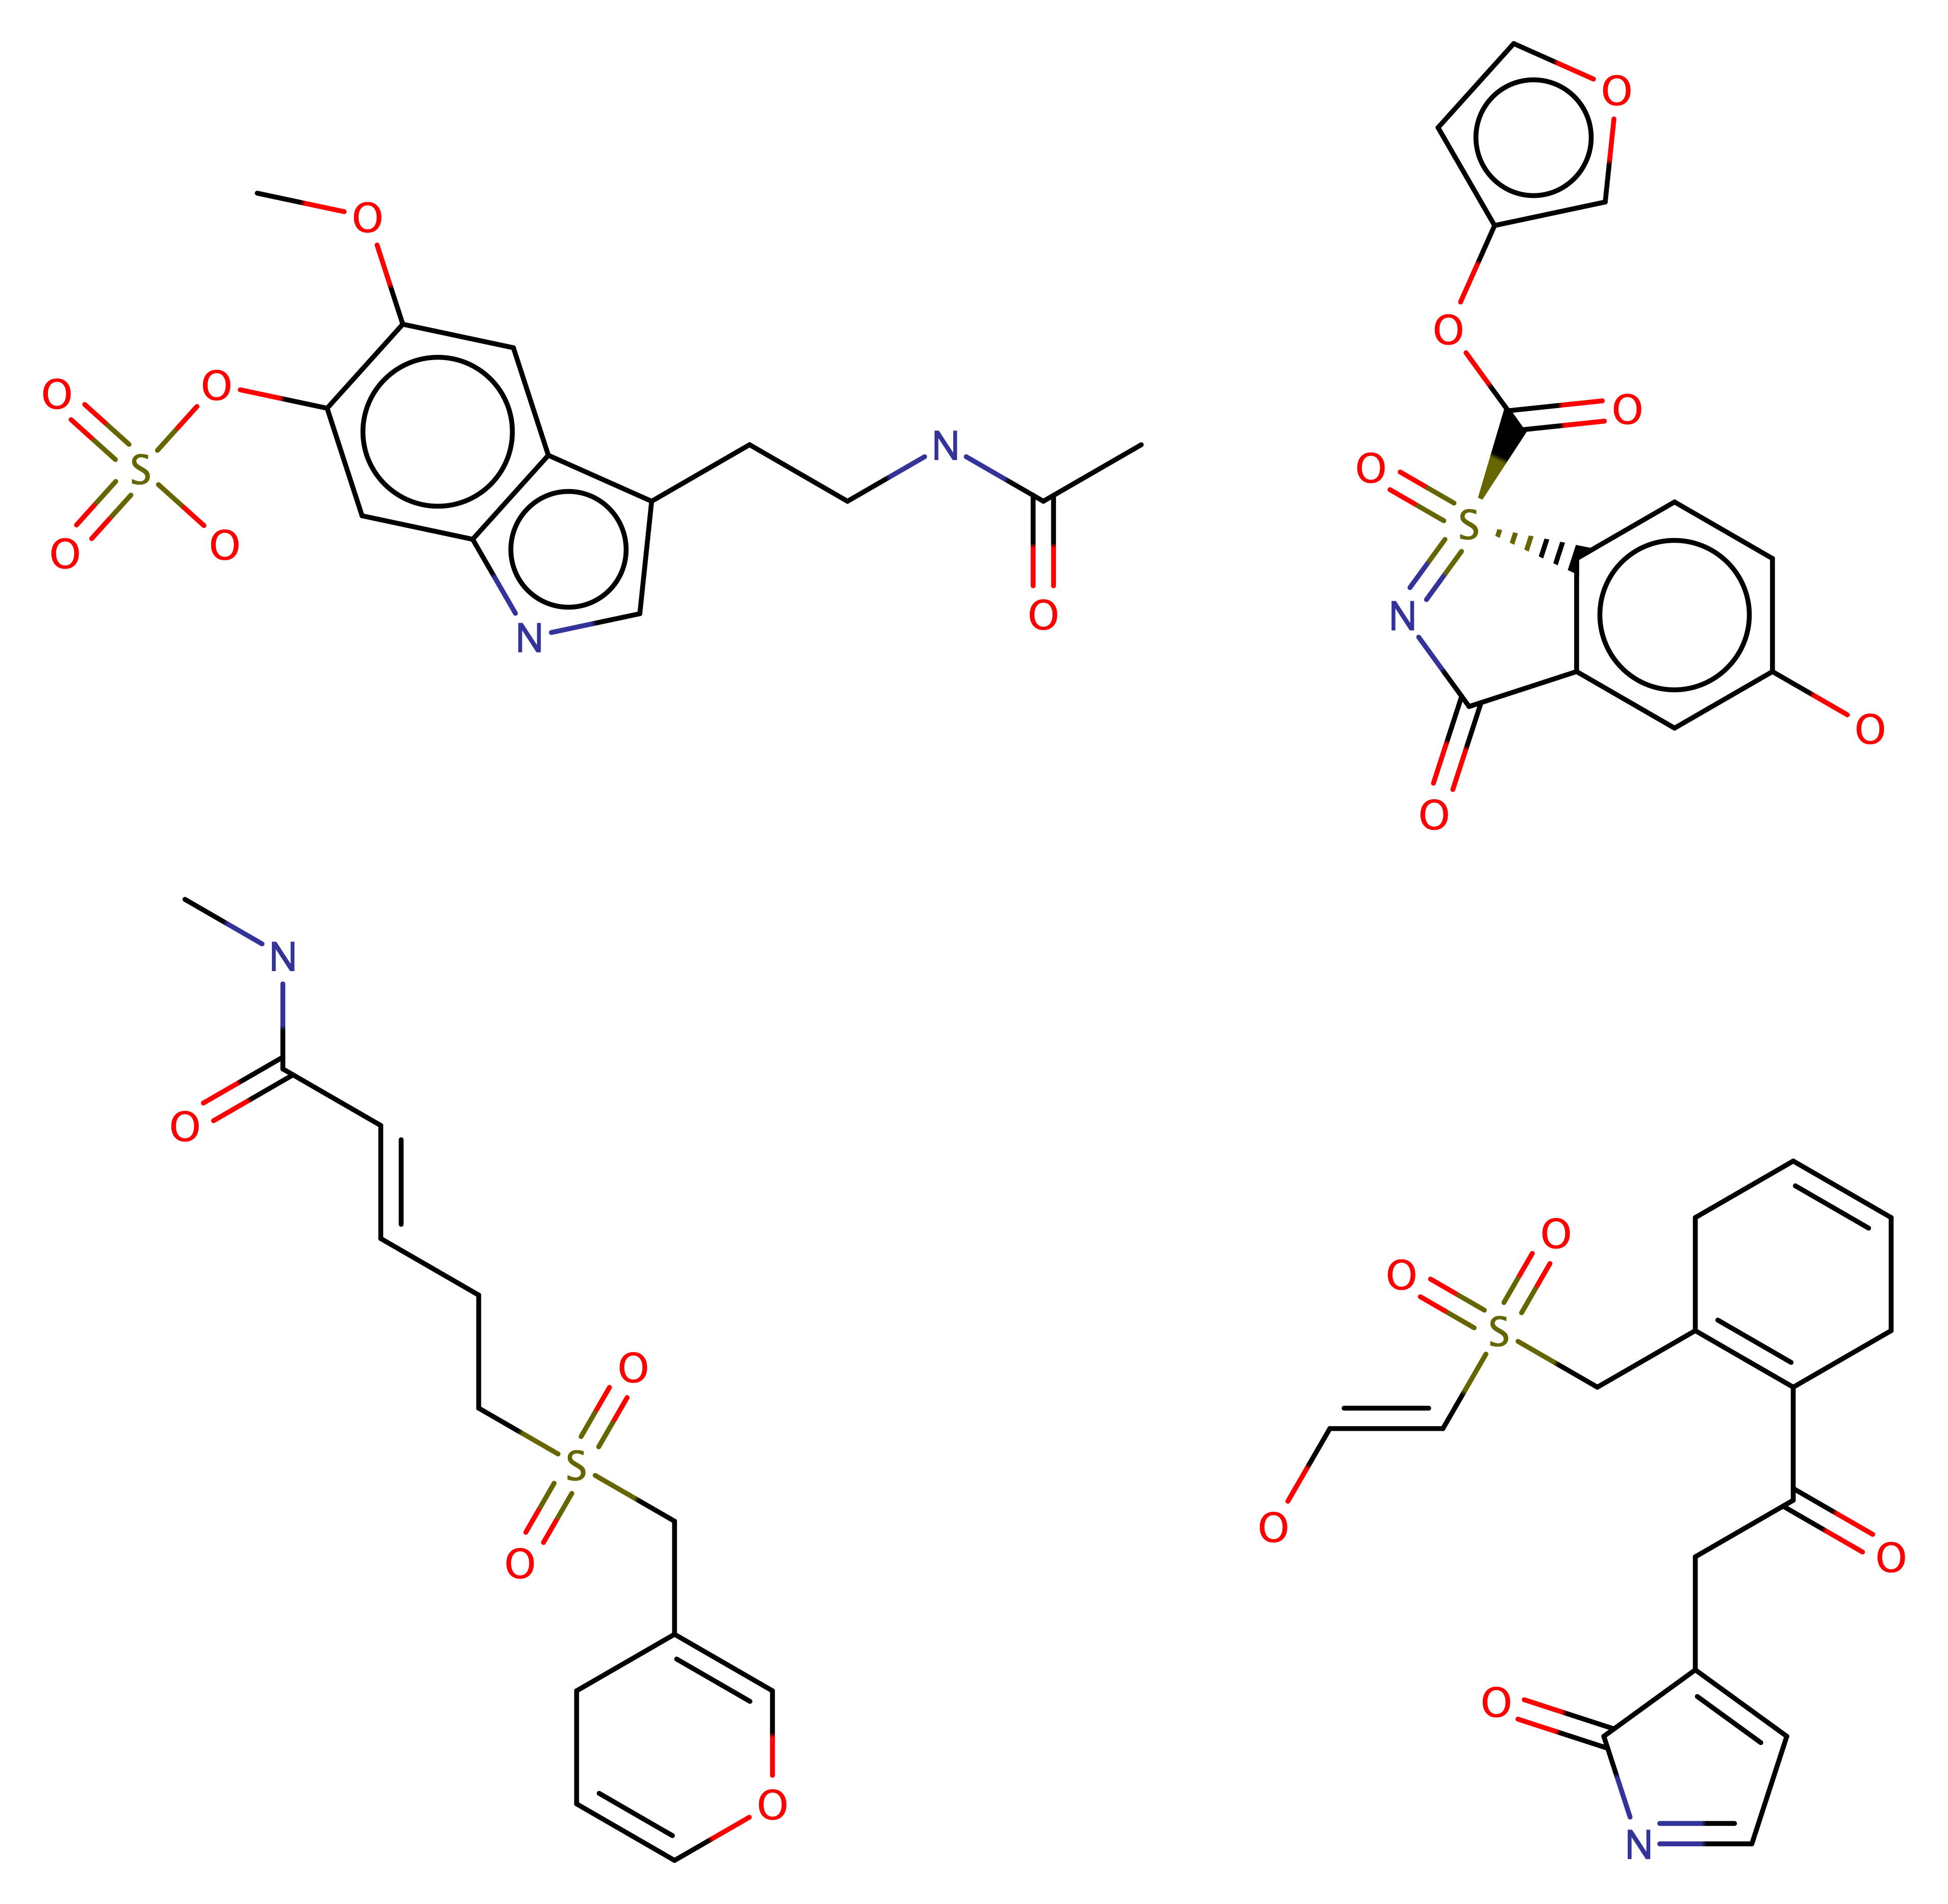
\includegraphics[width=0.5\textwidth]{Chapter3/Figs/GA_subs.png}
\caption{\label{fig:GA_subs} Several of the relatively chemically reasonable top-scoring candidates suggested by the SOAP genetic algorithm which were submitted to COVID Moonshot.}
\end{figure}

\begin{figure}[!h] % !h ~ force here, t ~ top, b ~ bottom, p ~ separate page
\centering
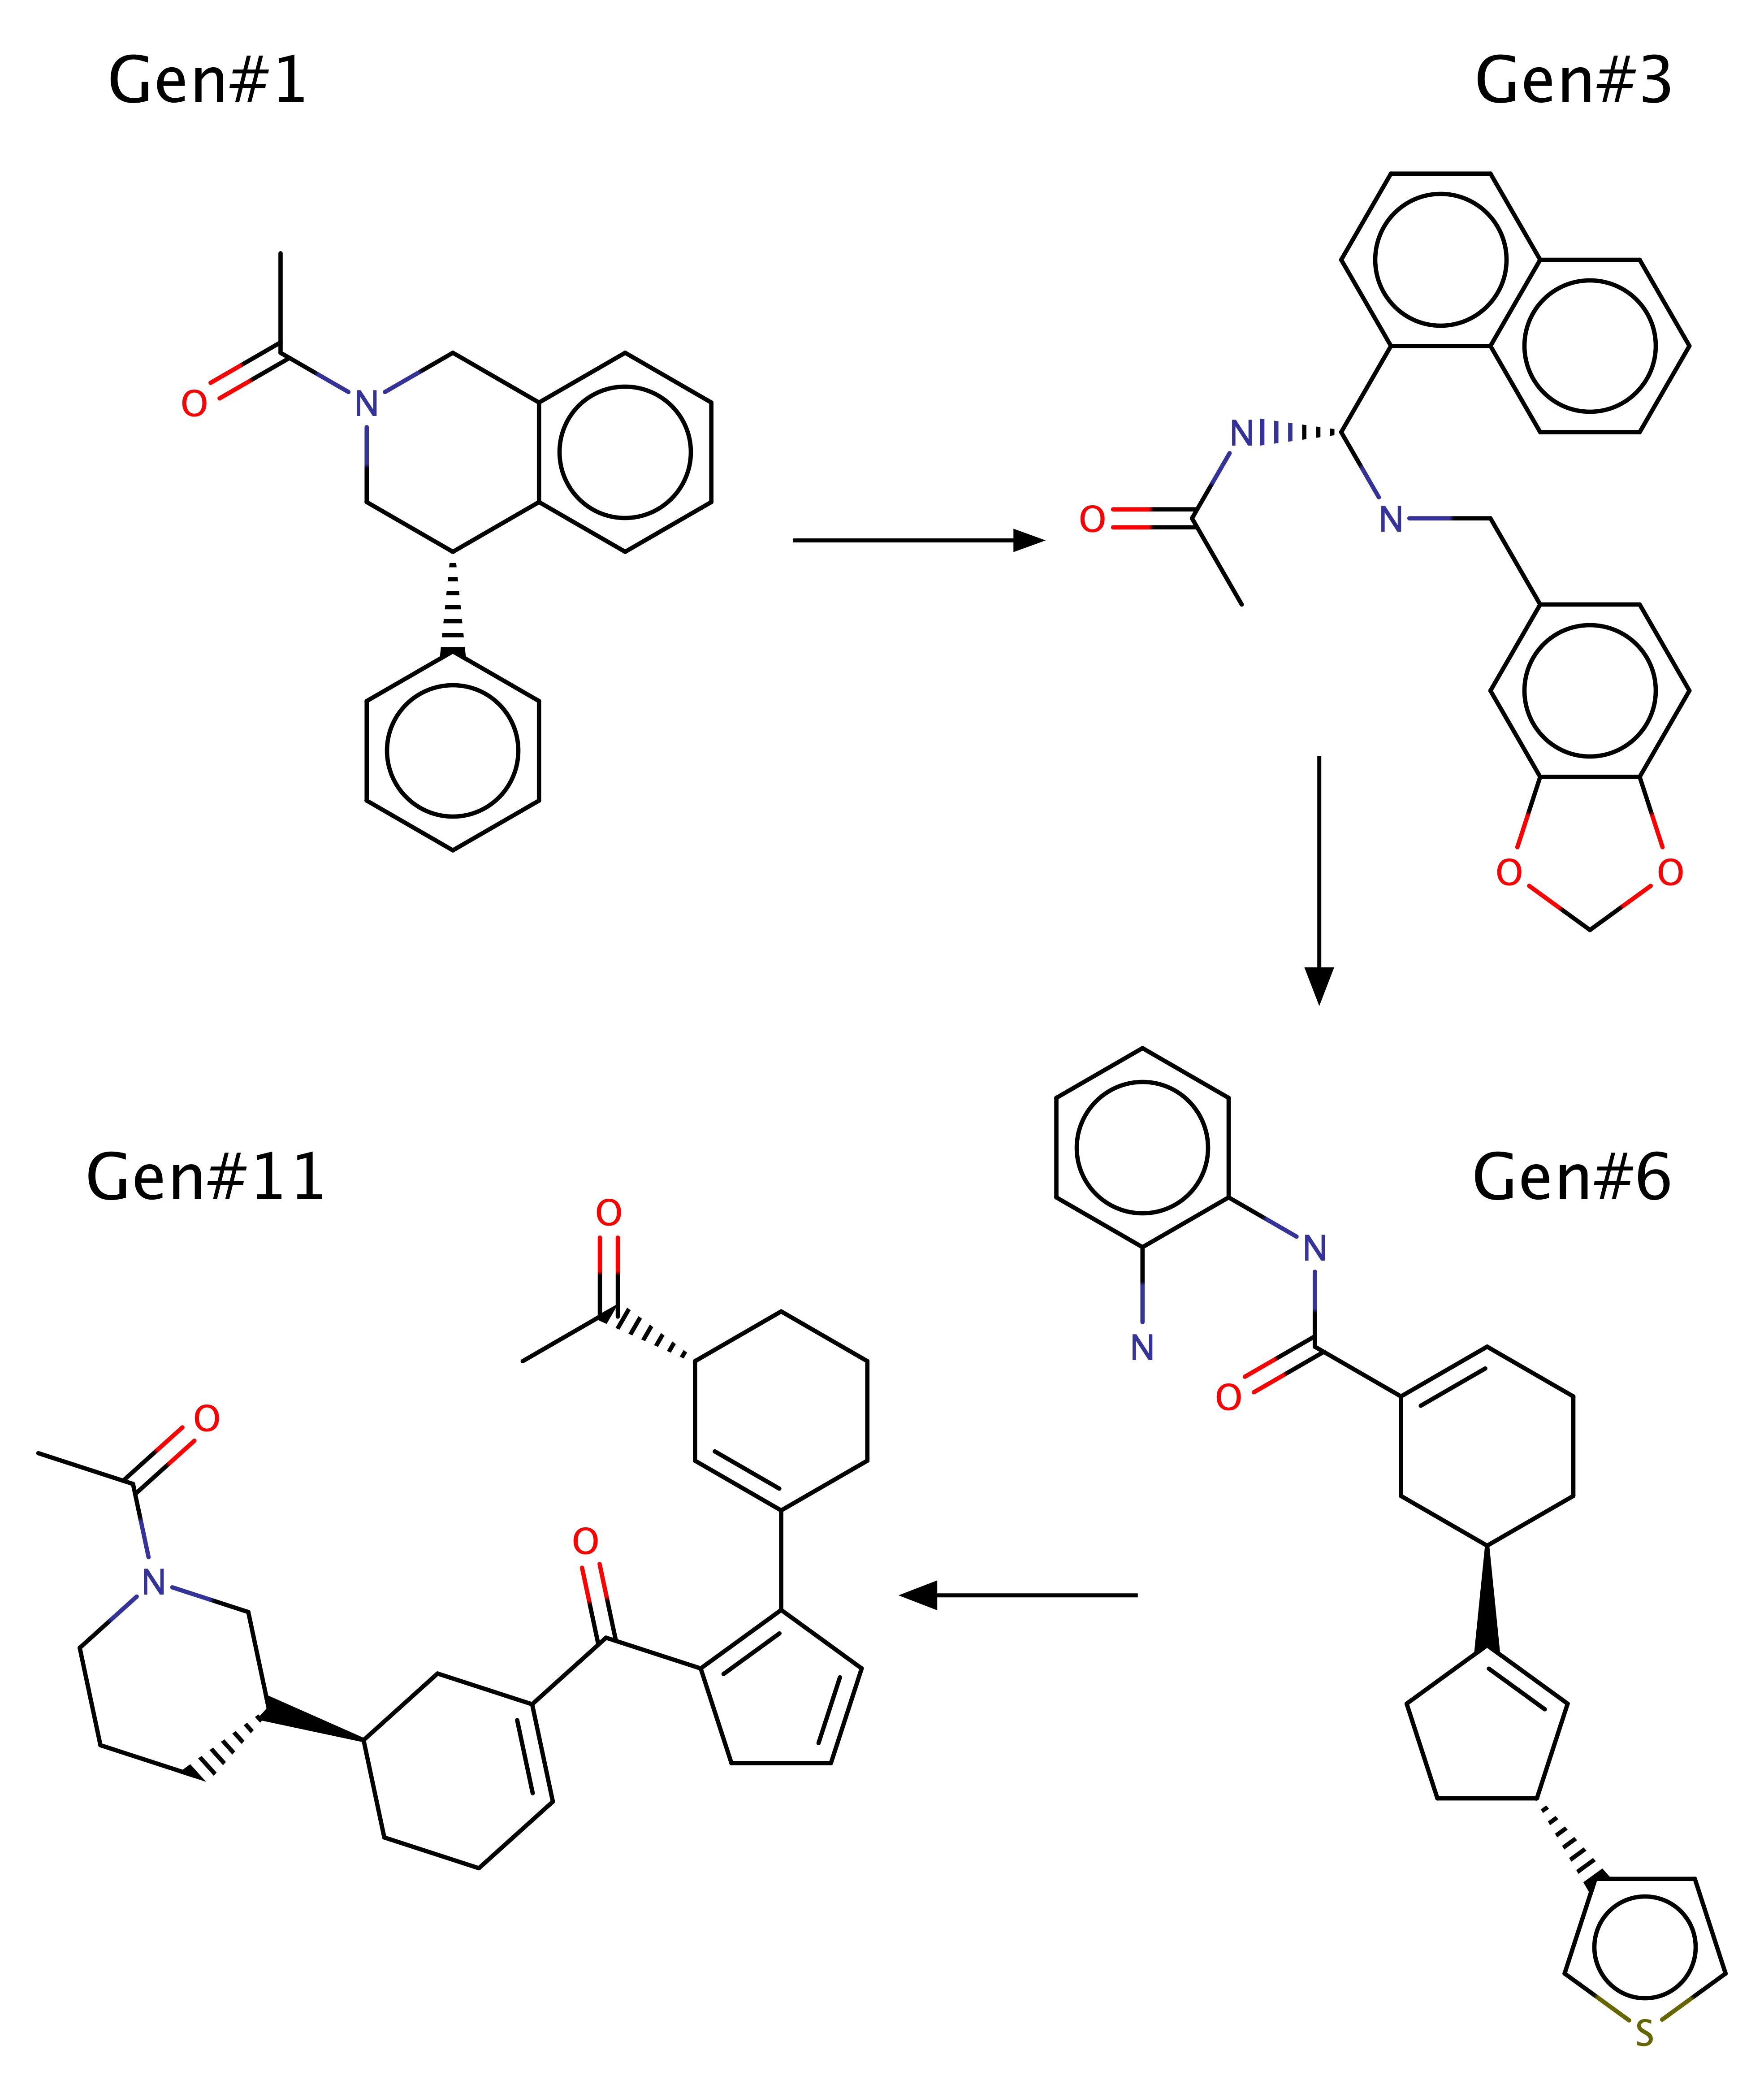
\includegraphics[width=0.5\textwidth]{Chapter3/Figs/GA.png}
\caption{\label{fig:GA_example} An example of the genetic evolution in size and complexity of the top-`scoring' candidate from a single run.}
\end{figure}

In hindsight, the fatal flaw of this approach was that the naive conformers generated by RDKit had no resemblance to the particular shape taken up by the bound fragment because of the horrendously complex molecular interactions between the molecule and the protein residues of the binding site. In addition, the inherently random nature of genetic algorithms (Fig.~\ref{fig:GA_example}) meant that the evolutionary candidates were often difficult to synthesize - ultimately, none of the submitted designs were made as limited financial resources led to the necessary triaging of candidates by synthesizability. Even if the resources were available to synthesize them, computational docking analysis gave a low score to these candidates, suggesting that it would have been unlikely that they would have been effective binders. It appears that a more targeted approach centered around synthesizable compounds would be necessary to warrant real-world impact.

\section{Series optimization}
In the most recent stage of the Moonshot initiative after synthesizing and assaying several hundred compounds, promising leads with $\mu$M-level IC50s were made. The research focus thus shifted from merely searching for active molecules, but to optimise the existing series to break through the $1\mu$M IC50 activity barrier.

The activity data collected up to that point could be split into three categories: acrylamide covalent inhibitors generated from chemical library of Ugi reaction products, chloroacetamide covalent inhibitors, and non-covalent inhibitors. The active molecules from all three series are known from crystallography data to bind to the same binding site in the protein target. In addition, there were also $\sim$180k datapoints from a High-Throughput Screen (HTS) of a chemical library, which are only single point inhibition measurements at $20\mu$M whereas the preceding data contained full dose-response curves. The threshold for classification as an active was achieving >50\% inhibition at $20\mu$M (Table \ref{table:actvitiy_table}).

\begin{table}[!h]
\caption{Available COVID Moonshot Activity Data}
\centering
\label{table:actvitiy_table}
\begin{tabular}{l c c}
\toprule
 Type & Size & Activity \\ 
\midrule
Chloroacetamides & 63 & 63\%  \\

Acrylamides & 179 & 15\%  \\

Non-covalents & 548 & 8\%  \\

HTS & 183,178 & 0.01\%  \\
\bottomrule
\end{tabular}
\end{table}

For achieving the objective of finding molecules that are better than existing candidates, a relatively simple workflow was adopted (Fig.~\ref{fig:pipe}). An ML scoring model as well as a method for generating drug candidates would be constructed from the activity data, with the top scoring candidates then triaged by synthesizability, made in real-life, and assayed by Moonshot.

\begin{figure}[!h] % !h ~ force here, t ~ top, b ~ bottom, p ~ separate page
\centering
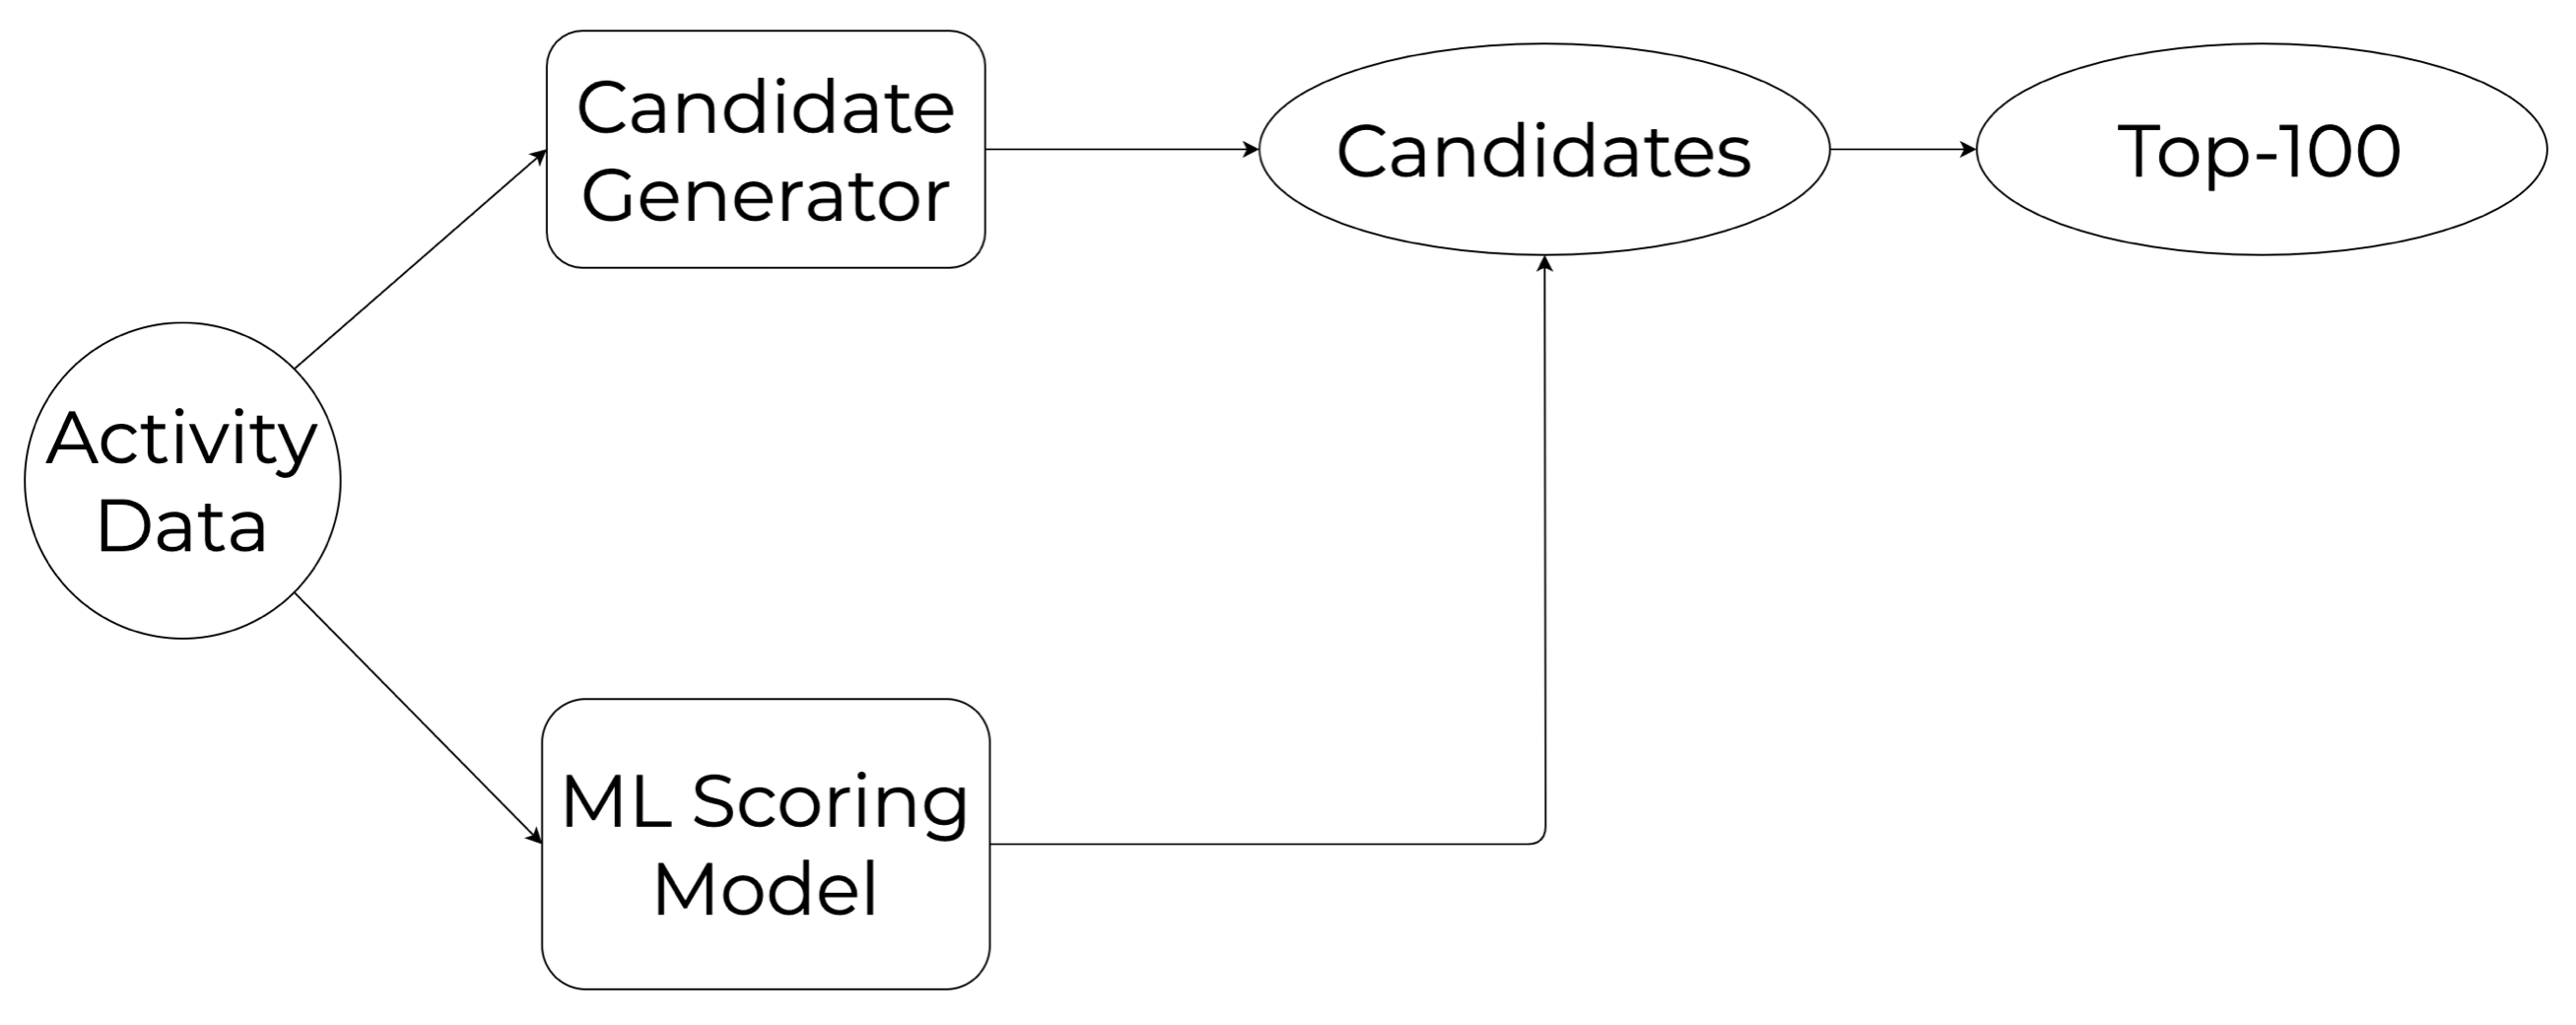
\includegraphics[width=\textwidth]{Chapter3/Figs/Moonshot_pipeline.png}
\caption{\label{fig:pipe} An illustration of the series optimisation pipeline.}
\end{figure}

\subsection{Multitask learning across chemical series}
Given the partitioning of the data, a multitask learning approach seemed most appropriate for constructing QSAR model. The idea behind multitask learning is to combine multiple loss functions from the prediction of each property so the model has to learn more generic features that are useful across multiple tasks, in essence acting as a form of regularization that improves predictive power \cite{zhang2017survey}. Particularly for this scenario, the value of learning to predict chloroacetamide activity and HTS inhibitions in isolation is low because the chloroacetamides are known to be very reactive and likely too toxic to be useful as a drug, while the HTS data is inherently quite noisy since the measurements are only at a single concentration. However, with multitask learning we can exploit the intrinsic information within the chloroacetamide and HTS data to improve QSAR performance on the acrylamides and non-covalents.

This approach was implemented using a particular graph neural network architecture known as a Message-Passing Neural Network (MPNN) model \cite{Gilmer17mpnn} chosen for its ease in implementation. The loss function for training was a sum of separate binary cross-entropy terms for active/inactive classification as well as mean-squared error terms for pIC50 regression of the active molecules for each task (apart from HTS which does not have pIC50 measurements). For performance evaluation, a stratified data split (same active/inactive proportion in train and test sets) was done on each series and the respective splits combined to form overall training and test sets. The performance of the model was compared to a baseline random-forest model trained using Morgan fingerprint features, as well as an MPNN without multitasking, and an MPNN multitasking without the HTS data. The classification results are detailed in Table \ref{table:multitask_table}.

\begin{table}[!h]
\caption{Multitask QSAR classification results - 5 runs, random stratified split}
\centering
\label{table:multitask_table}
\begin{tabular}{lcccccc}
\toprule
\multirow{2}{*}{Model} & \multicolumn{2}{c}{Acryl.} & \multicolumn{2}{c}{Chloro.} & \multicolumn{2}{c}{Non-cov.}\\ 
\cmidrule(lr){2-3} \cmidrule(lr){4-5} \cmidrule(lr){6-7}
  & ROC & PRC  & ROC & PRC & ROC & PRC \\ 
\midrule
Random Forest & 0.7 & 0.45 & 0.8 & 0.8 & 0.7 & 0.2 \\

MPNN - Single & 0.7 & 0.4 & 0.8 & 0.8 & 0.65 & 0.2 \\

MPNN - Multi & 0.7 & 0.5 & 0.85 & 0.8 & 0.75 & 0.3 \\

MPNN - Multi + HTS & \textbf{0.8} & \textbf{0.5} & \textbf{0.9} & \textbf{0.85} & \textbf{0.85} & \textbf{0.5} \\
\bottomrule
\end{tabular}
\end{table}

The results clearly show the impact of multitask learning - sharing information across tasks allows the MPNN to outperform the robust random forest baseline on all tasks. The observation that including the HTS results greatly boost predictive power for the non-covalents suggests that the majority of actives in the HTS dataset are also non-covalent inhibitors.

Although the models above were able to reliably classify molecules as active/inactive, all of them failed on the regression of pIC50s, frequently making poor predictions (negative $R^{2}$ correlation on test sets). This is attributed to the much lower number of regression datapoints due to the sparseness of activity, as well as the fact that learning to regress pIC50s is a genuinely hard task. Unfortunately, this suggests that with this approach the model can only learn to classify activity but is unable to rank the activity.

\subsection{Learning pairwise ranking with siamese networks}
Returning to the objective of this task, the goal is to find molecules that are more active, not merely classifying as active/inactive. Instead of formulating the task as a QSAR problem, an alternative line of attack is to consider pairwise ranking - given a pair of molecules $(A,B)$, is $A$ more active than $B$? This approach effectively combines `easy' classification and `difficult' regression into one `moderate' ranking task - binary classification of input pairs. In machine learning, this type of task is handled using models known as Siamese Neural Networks (SNNs) \cite{Koch2015SiamneseNN} where the the two inputs are encoded in the same way before their hidden states are operated on in unison to make a prediction. With a trained SNN, for scoring a drug candidate $X$ we can use the model prediction for $(X,Z)$ where $Z$ is the most potent active in the dataset.

The SNN architecture that was used for this task also utilizes MPNNs (Fig \ref{fig:snn}). Both molecules from the input pair are passed through the same MPNN encoder to obtain their learnt graph embedding vectors; several fully-connected layers then operate on the vector difference between the graph embeddings to make the classification prediction. To enforce the antisymmetry of the model (so that $f(X,Y) = 1 - f(Y,X)$), all layer activations are tanh functions and the linear layers do not have any bias terms.
\begin{figure}[!h] % !h ~ force here, t ~ top, b ~ bottom, p ~ separate page
\centering
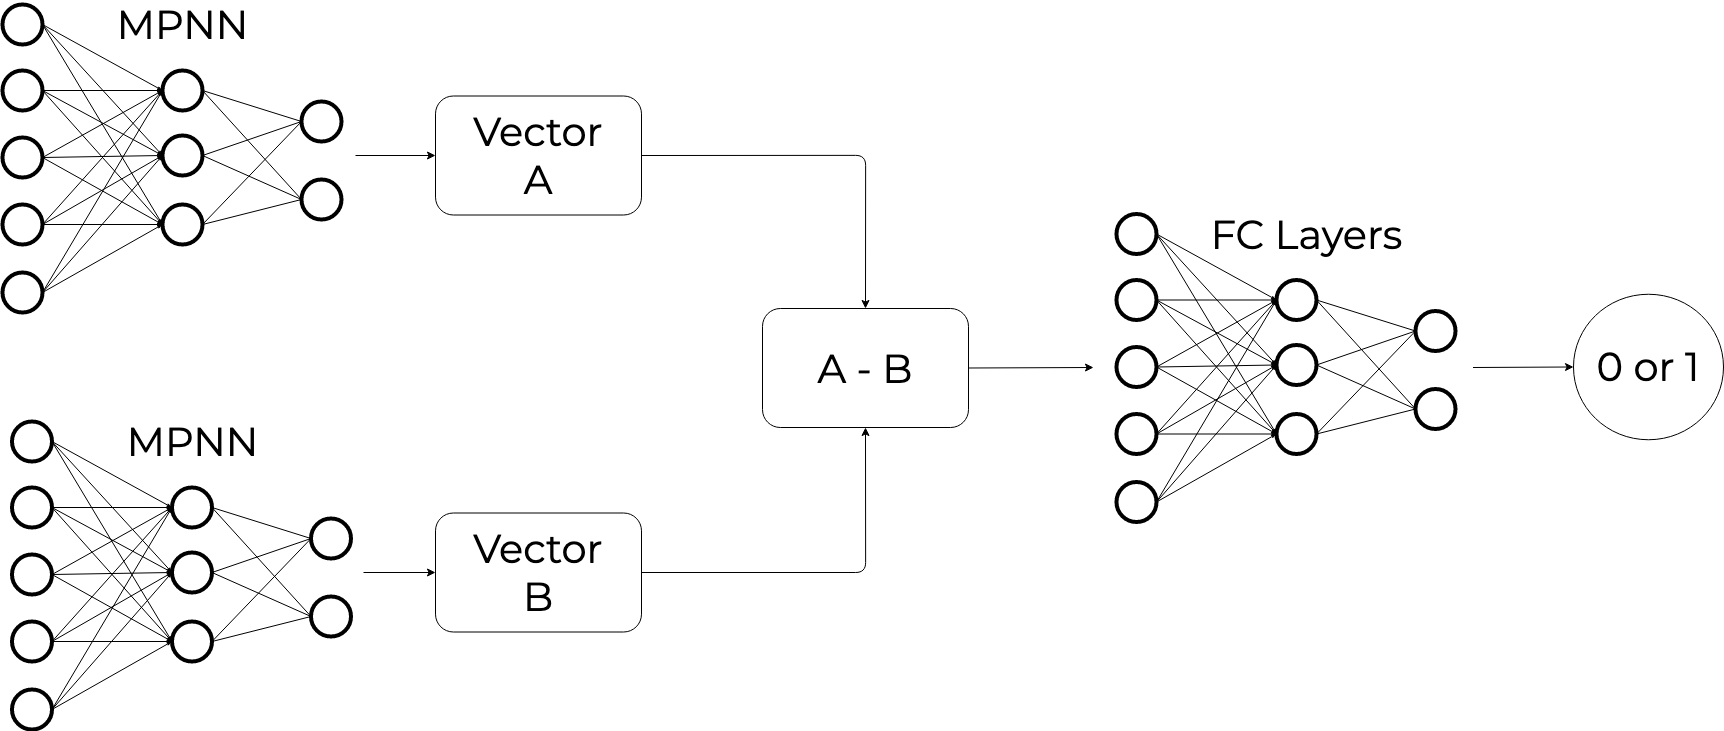
\includegraphics[width=\textwidth]{Chapter3/Figs/SNN.png}
\caption{\label{fig:snn} An illustration of how the Siamese MPNN model is implemented.}
\end{figure}

To construct a suitable dataset for training the SNN, the activity data must be reformated into molecular pairs. This was done by pairing all actives with all inactives within each series, as well as pairing up actives where there is a significant activity difference ($\Delta$IC50 $>5\mu$M). The inactive molecules were not paired up between each other as the ranking of inactivity is not relevant to the task at hand and potentially noisy/misleading. The HTS data is also left out as the sheer size of that dataset leads to a computationally unfeasible number of molecular pairs even if the pairing is constrained by Tanimoto similarity. 

A flipped pairing is included for all pairs so that the dataset is antisymmetric since the model would just predict ones otherwise. Theoretically this method is appealing because it is a natural way of oversampling the low proportion of actives, addressing the problem of dataset imbalance commonly seen in drug discovery classification tasks. Additionally, creating pairs between the actives allows the exploitation of activity information without the noise/difficulty of trying to learn accurate pIC50 values. In this set-up there is only one single binary classification task, however the beneficial regularization from multitask learning remain as the model still has to reliably rank activity on all three series.

For performance evaluation, train and test sets were split (again with the same active/inactive proportion for each series) to contain a disjoint set of molecules before the molecules are paired up independently within each set. This ensures that there is no cross-talk between the train/test sets where the model could simply memorize the activity of certain compounds. The pairwise classification performance for each series are shown in Table \ref{table:pairwise_table}.

\begin{table}[!h]
\caption{Graph SNN pairwise ranking results}
\centering
\label{table:pairwise_table}
\begin{tabular}{l c c}
\toprule
 Series & ROC-AUC & PRC-AUC \\ 
\midrule
Chloroacetamides & 0.80 & 0.71  \\

Acrylamides & 0.78 & 0.80 \\

Non-covalents & 0.74 & 0.74 \\
\bottomrule
\end{tabular}
\end{table}

The performance metrics indicate that the model is able to reliably classify whether one compound is more active than another, in particular with much better precision-recall than seen in simply classifying activity.

\subsection{Construction of screening library}
After designing a well-founded ML scoring model, a list of candidate molecules must be generated to rank by score. Many ML methods for candidate generation have been described in the literature, ranging from relatively straightforward applications of distribution-learning ML models such as Variational Auto-Encoders \cite{Bombarelli2018VAE}, to more chemistry-tailored approaches such as scaffold decoration \cite{Pous2020scaffold}. While at first glance these seem ideal for the task at hand, attempting to implement these in practice reveal that these methods tend to generate molecules that are not particularly goal-orientated, ignoring prior chemical intuition regarding the scaffold of the active molecules. Presumably this is addressed in more complex molecular generative workflows where a scoring model is incorporated in a Reinforcement Learning feedback loop \cite{born2019paccmannrl}; due to time constraints this was not investigated.

Instead, a more traditional method of constructing and screening an explicit chemical library was chosen. The general approach for generating the chemical library is by decomposing the existing compounds into distinct components before enumerating all components with one another, all according to manually specified rules based on chemical intuition. Separate libraries were generated for the acrylamides and the non-covalents as the prior known intuitions and ease of synthesizability for those two series are different. In this case, it was observed that a unifying motif for many of the active molecules was the presence of an amide or urea group in the central part of the scaffold (Fig \ref{fig:example}). The presence of amides is unsurprising since they are guaranteed to appear in the products of the Ugi reaction but they are also frequent in the non-covalents. 

\begin{figure}[!h] % !h ~ force here, t ~ top, b ~ bottom, p ~ separate page
\centering
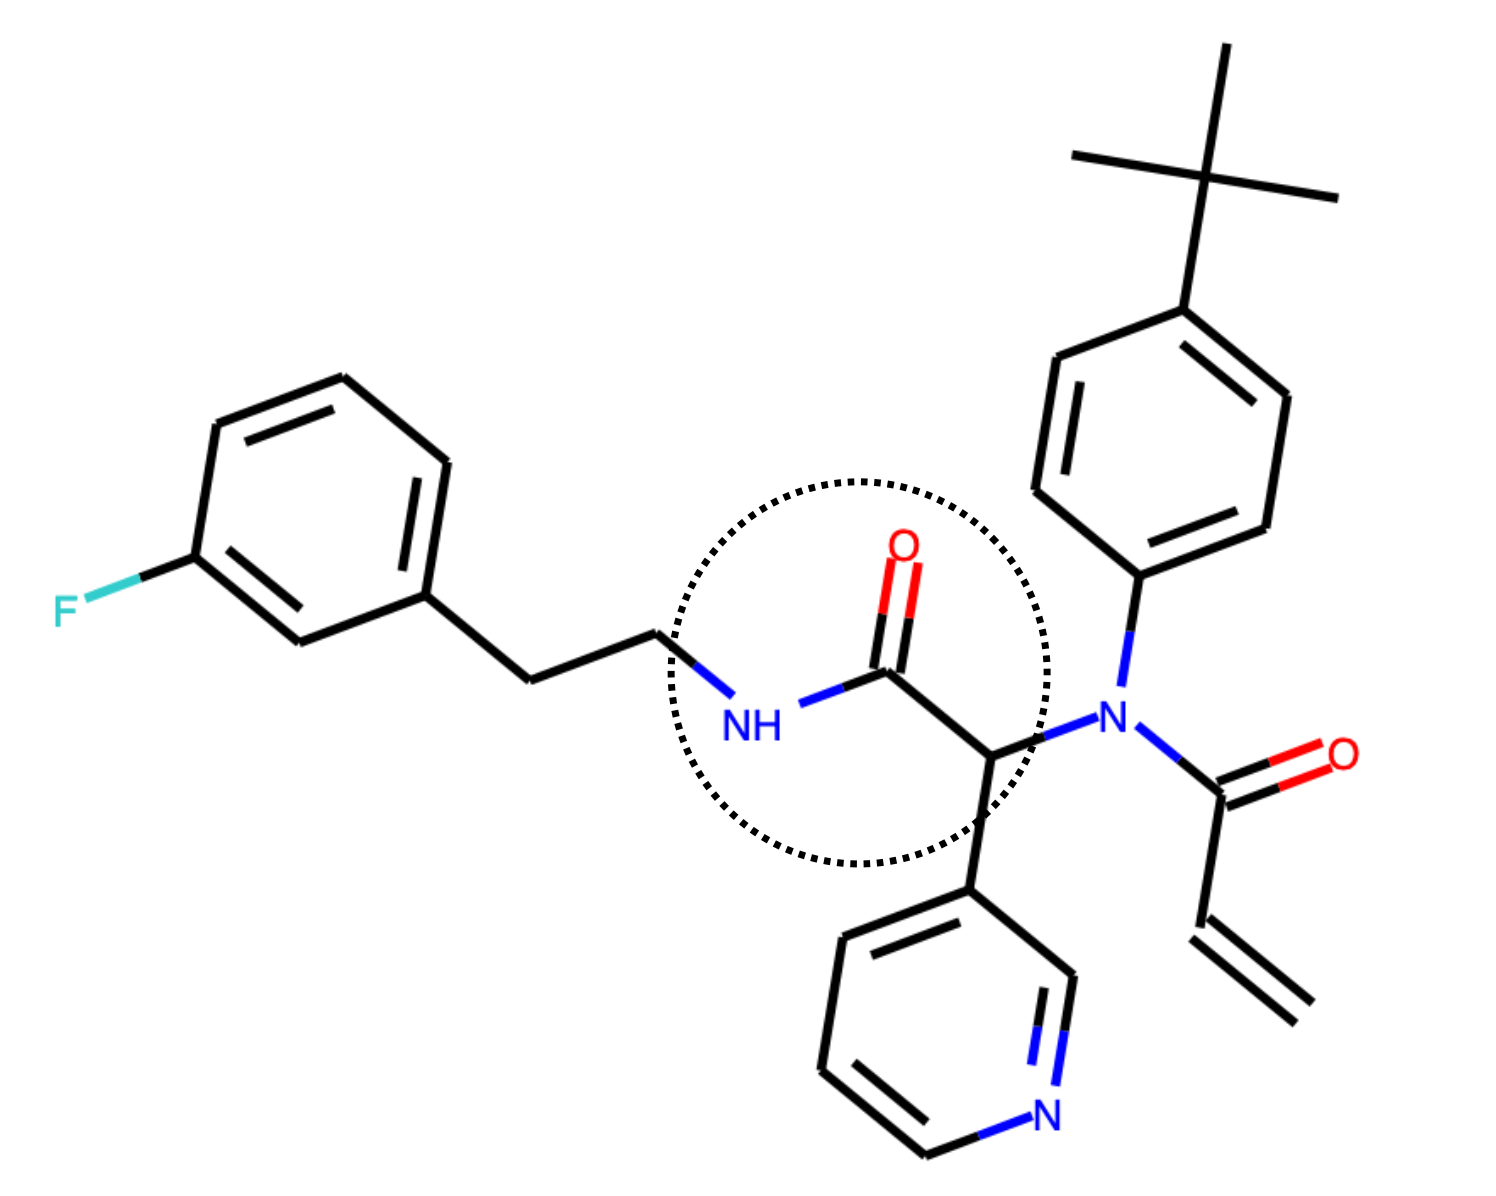
\includegraphics[width=0.5\textwidth]{Chapter3/Figs/example_mol.png}
\caption{\label{fig:example} An example of a potent molecule (IC50 = $2.96\mu$M) where the amide/urea motif is highlighted with the dashed circle.}
\end{figure}

For the non-covalents, the procedure was therefore to slice along all amide and urea bonds as well as the slicing the substituents from secondary amines. All possible secondary amines were then enumerated by combining all substituents with all primary amines, and all primary/secondary amines were then combined with all substituents to obtain a library of amides and ureas. This resulted in a library of size $\sim$870k. For the acrylamides the procedure is more straightforward, simply being an enumeration of all possible Ugi reaction components (carboxylic acids, primary amines, ketone/aldehydes, and isocyanides) in the dataset. The primary amines derived from the non-covalents were also included in the enumeration process, resulting in a library of size $\sim$11k. 

\subsection{Preliminary Results}
An ensemble of 5 SNNs were trained on the full dataset of (inactive-active) and (active-more active) molecular pairs. The models then predicted the activity of both libraries relative to each of the top-4 most potent actives within the non-covalent and acrylamide series. The 4 predictions for each molecule were averaged, and the ensemble average of that was used to score the molecules. The resultant top-100 candidates from each library were submitted to the COVID Moonshot team to triage by synthesizability and chemical novelty. Out of the 200 proposed molecules, 4 non-covalent candidates and 2 acrylamides were chosen to be made and tested in real life. These molecules along with their most similar (as measured by Tanimoto similarity) assayed analogue from the training set of the Siamese networks are shown in Fig.~\ref{fig:moonshot_subs}.

\begin{figure}[!h] % !h ~ force here, t ~ top, b ~ bottom, p ~ separate page
\centering
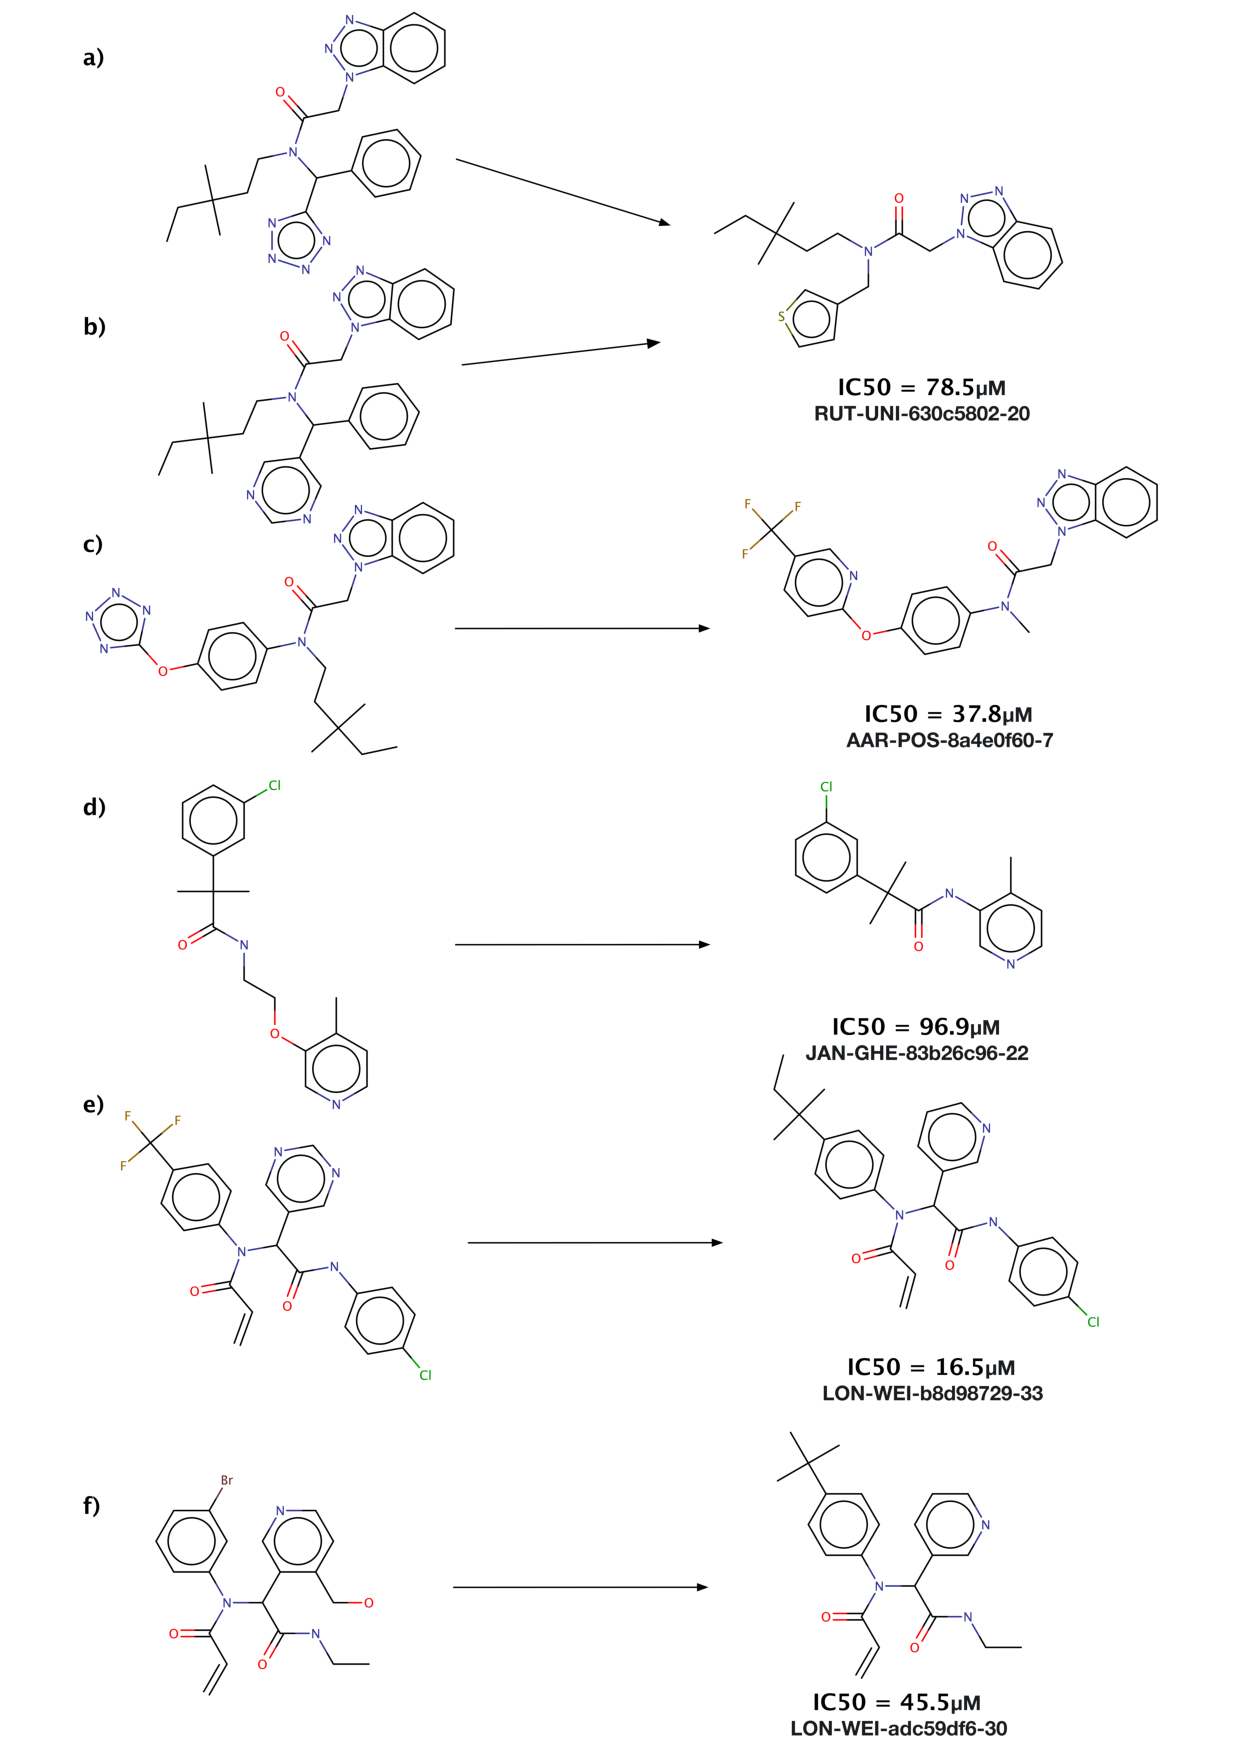
\includegraphics[width=0.9\textwidth]{Chapter3/Figs/all_subs.pdf}
\caption{\label{fig:moonshot_subs} Submitted drug candidates and their most similar analogue in the training set -- the model predictions consist of a small, reasonable numer of chemical modifications to existing, known active molecules.}
\end{figure}

Molecules a)-d) were submitted on July 13th while e)-f) were submitted on July 24th. At the time of writing only molecule d) has been synthesized and tested. This molecule was unfortunately inactive (IC50>99.5$\mu$M) as measured with both Fluorescence and Rapidfire inhibition measurements. However the closest analogue to this molecule in the training set has relatively low activity (96.9$\mu$M) so this is not too surprising. Results for the other submissions are being awaited with cautious optimism.